%%%%%%%%%%%%%%%%%%%%%%%%%%%%%%%%%%%%%%%%%%%%%%%%%%%%%%%%%%%%%%%%%%%%%%%%%%%%%%%%%%%%%%%%%%%%%%%%%%%%%%
%
%   Filename    : appendix_A.tex 
%
%   Description : This file is for including the Research Ethics Documents (delegated as Appendix A) 
%                 
%%%%%%%%%%%%%%%%%%%%%%%%%%%%%%%%%%%%%%%%%%%%%%%%%%%%%%%%%%%%%%%%%%%%%%%%%%%%%%%%%%%%%%%%%%%%%%%%%%%%%%

\chapter{Figures and Tables}
\label{sec:appendixa}



% Save the file you want to include in PDF format.
% Uncomment the commant below specifying the correct appendix file. 
%\includepdf[pages=-, scale = 0.9, pagecommand={}, offset = -30 0]{appendixA.pdf}

\begin{figure}
	\caption{Code snippet of the prototype}
	\centering
	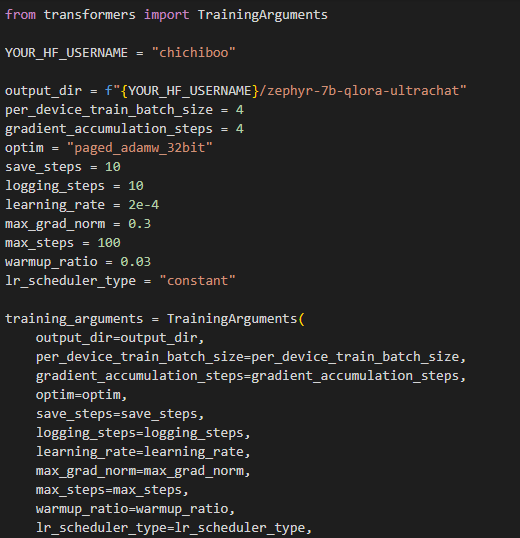
\includegraphics{figures/qlora-snippet}
\end{figure}

\begin{table}[h!]
	\caption{Difference between Generated Answers of the Base and LoRA Fine-Tuned Model} \vspace{0.25em}
	\centering
	\renewcommand{\arraystretch}{1.2} % Adjusts row spacing
	\begin{tabular}{@{}lp{0.85\linewidth}@{}}
		\hline
		\textbf{Before LoRA:} & \\
		USER: & Can you explain contrastive learning in machine learning in simple terms for someone new to the field of ML? \\
		ASSISTANT: & Contrastive learning is a machine learning technique that involves training a model to learn from data that is similar to the target data. The model is trained to identify patterns in the data that are similar to the target data, and to use those patterns to make predictions about new data. \\
		\hline
		\textbf{After LoRA:} & \\
		USER: & Can you explain contrastive learning in machine learning in simple terms for someone new to the field of ML? \\
		ASSISTANT: & Contrastive learning is a technique in machine learning that uses a technique called contrastive loss to train a model. The idea is to train a model to distinguish between similar and dissimilar data. In contrastive learning, a model is trained to distinguish between a pair of similar data, such as a pair of images, and a pair of dissimilar data, such as a pair of different images. The model is trained to minimize the loss, which is the difference between the similarity and dissimilarity of the data. In contrast, traditional machine learning techniques, such as supervised learning, are trained to distinguish between different types of data, such as a classification or regression task. In summary, contrastive learning is a technique in machine learning that uses a technique called contrastive loss to train a model to distinguish between similar and dissimilar data, which is different from traditional machine learning techniques, such as supervised learning. \\
		\hline
	\end{tabular}
\end{table}
